\documentclass[a4paper,12pt]{article}

\usepackage{fancyhdr}
\pagestyle{fancy}
\fancyhf{}
\rhead{Dominic Moylett - dm1905@my.bristol.ac.uk}
\cfoot{Page \thepage}

\usepackage{tikz}
\usetikzlibrary{positioning}

\usepackage{circuitikz}

\usepackage{amsmath}

\begin{document}
    \begin{center}
        \section*{Fault Tolerant Computing and VLSI Testing}
        \subsection*{Assignment 3}
    \end{center}

    \begin{enumerate}

        \item The Markov Model for the system with self-diagnostics is:

            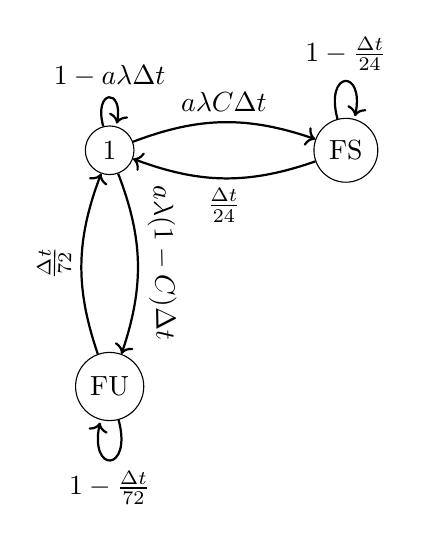
\begin{tikzpicture}[node distance=3cm]
                \tikzset{state/.style={draw, shape=circle}}
                \node[state] (1) at (0, 0) {1};
                \node[state, right of = 1] (FS) {FS};
                \node[state, below of = 1] (FU) {FU};
                \path[->, thick]
                    (1) edge [loop above] node {$1 - a\lambda\Delta t$} (1)
                        edge [bend left = 20] node [above] {$a\lambda C\Delta t$} (FS)
                        edge [bend left = 20] node [above, sloped] {$a\lambda(1 - C)\Delta t$} (FU)
                    (FS) edge [loop above] node {$1 - \frac{\Delta t}{24}$} (FS)
                        edge [bend left = 20] node [below] {$\frac{\Delta t}{24}$} (1)
                    (FU) edge [loop below] node {$1 - \frac{\Delta t}{72}$} (FU)
                        edge [bend left = 20] node [above, sloped] {$\frac{\Delta t}{72}$} (1);
            \end{tikzpicture}

            \begin{itemize}
                \item 1 is where the system is working successfully.
                \item FS is where a fault has been detected and the system has been safely deactivated.
                \item FU is where a fault has not been detected.
            \end{itemize}

            $P(t) = \begin{bmatrix} P_1(t) \\ P_{FS}(t) \\ P_{FU}(t) \\ \end{bmatrix}, P_1(t) + P_{FS}(t) + P_{FU}(t) = 1, P(0) = \begin{bmatrix} 1 \\ 0 \\ 0 \end{bmatrix}$

            $A = \begin{bmatrix}
                1 - a\lambda\Delta t    & \frac{\Delta t}{24}     & \frac{\Delta t}{72}     \\
                a\lambda C\Delta t      & 1 - \frac{\Delta t}{24} & 0                       \\
                a\lambda(1 - C)\Delta t & 0                       & 1 - \frac{\Delta t}{72} \\
            \end{bmatrix}$ 

            $P(t + \Delta t) = AP(t) = \begin{bmatrix}
                P_1(t)(1 - a\lambda\Delta t) + P_{FS}(t)\frac{\Delta t}{24} + P_{FU}(t)\frac{\Delta t}{72} \\
                P_1(t)a\lambda C\Delta t + P_{FS}(t)(1 - \frac{\Delta t}{24}) \\
                P_1(t)a\lambda(1 - C)\Delta t + P_{FU}(t)(1 - \frac{\Delta t}{72}) \\
            \end{bmatrix}$

            $P_1(t + \Delta t) = P_1(t)(1 - a\lambda\Delta t) + P_{FS}(t)\frac{\Delta t}{24} + P_{FU}(t)\frac{\Delta t}{72}$

            $P_{FS}(t + \Delta t) = P_1(t)a\lambda C\Delta t + P_{FS}(t)(1 - \frac{\Delta t}{24})$

            $P_{FU}(t + \Delta t) = P_1(t)a\lambda(1 - C)\Delta t + P_{FU}(t)(1 - \frac{\Delta t}{72})$

            $\frac{P_1(t + \Delta t) - P_1(t)}{\Delta t} = - P_1(t)a\lambda + \frac{P_{FS}(t)}{24} + \frac{P_{FU}(t)}{72}$

            $\frac{P_{FS}(t + \Delta t) - P_{FS}(t)}{\Delta t} = P_1(t)a\lambda C - \frac{P_{FS}(t)}{24}$

            $\frac{P_{FU}(t + \Delta t) - P_{FU}(t)}{\Delta t} = P_1(t)a\lambda(1 - C) - \frac{P_{FU}(t)}{72}$

            As $\Delta t\to 0$:

            $\frac{dP_1(t)}{dt} = - P_1(t)a\lambda + \frac{P_{FS}(t)}{24} + \frac{P_{FU}(t)}{72}$

            $\frac{dP_{FS}(t)}{dt} = P_1(t)a\lambda C - \frac{P_{FS}(t)}{24}$

            $\frac{dP_{FU}(t)}{dt} = P_1(t)a\lambda(1 - C) - \frac{P_{FU}(t)}{72}$

            The Markov Model for the system without self-diagnostics is:

            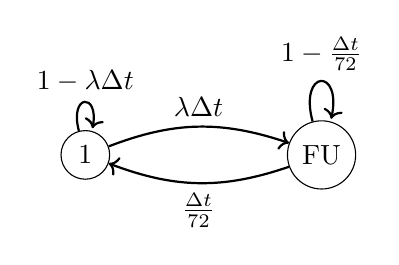
\begin{tikzpicture}[node distance=3cm]
                \tikzset{state/.style={draw, shape=circle}}
                \node[state] (1) at (0, 0) {1};
                \node[state, right of = 1] (FU) {FU};
                \path[->, thick]
                    (1) edge [loop above] node {$1 - \lambda\Delta t$} (1)
                        edge [bend left = 20] node [above] {$\lambda\Delta t$} (FU)
                    (FU) edge [loop above] node {$1 - \frac{\Delta t}{72}$} (FU)
                        edge [bend left = 20] node [below] {$\frac{\Delta t}{72}$} (1);
            \end{tikzpicture}

            \begin{itemize}
                \item 1 is where the system is working successfully.
                \item FU is where a fault has occured.
            \end{itemize}

            $P(t) = \begin{bmatrix} P_1(t) \\ P_{FU}(t) \end{bmatrix}, P_1(t) + P_{FU}(t) = 1, P(0) = \begin{bmatrix} 1 \\ 0 \end{bmatrix},$
            $A = \begin{bmatrix}
                1 - \lambda\Delta t && \frac{\Delta t}{72}     \\
                \lambda\Delta t     && 1 - \frac{\Delta t}{72} \\
            \end{bmatrix}$

            $P(t + \Delta t) = AP(t) = \begin{bmatrix}
                P_1(t)(1 - \lambda\Delta t) + P_{FU}(t)\frac{\Delta t}{72}       \\
                P_1(t)\lambda\Delta t       + P_{FU}(t)(1 - \frac{\Delta t}{72}) \\
            \end{bmatrix}$

            $\frac{P_1(t + \Delta t) - P_1(t)}{\Delta t} = -P_1(t)\lambda + \frac{P_{FU}(t)}{72},$
            $\frac{P_{FU}(t + \Delta t) - P_FU(t)}{\Delta t} = P_1(t)\lambda - \frac{P_{FU}(t)}{72}$

            As $\Delta t \to 0$:

            $\frac{dP_1(t)}{dt} = -P_1(t)\lambda + \frac{P_{FU}(t)}{72},$
            $\frac{dP_{FU}(t) }{dt} = P_1(t)\lambda - \frac{P_{FU}(t)}{72}$

            $sP_1(s) + sP_{FU}(s) = 1 \implies P_{FU}(s) = \frac{1 - sP_1(s)}{s}$

            $sP_1(s) - P_1(0) = sP_1(s) - 1 = -P_1(s)\lambda + \frac{P_{FU}(s)}{72} = -P_1(s)\lambda + \frac{1 - sP_1(s)}{72s}$

            $s^2P_1(s) - s = -sP_1(s)\lambda + \frac{1 - sP_1(s)}{72}$

            $s^2P_1(s) + sP_1(s)\lambda + \frac{sP_1(s)}{72} = sP_1(s)(s + \lambda + \frac{1}{72}) = s + \frac{1}{72}$

            $P_1(s) = \frac{s + \frac{1}{72}}{(s)(s + \lambda + \frac{1}{72})}$

            We can solve this equation via partial fractions:

            $P_1(s) = \frac{s + \frac{1}{72}}{(s)(s + \lambda + \frac{1}{72})} = \frac{A}{s} + \frac{B}{s + \lambda + \frac{1}{72}} \implies A(s + \lambda + \frac{1}{72}) + Bs = s + \frac{1}{72}$

            $s = 0 \implies A(\lambda + \frac{1}{72}) = \frac{1}{72} \implies A = \frac{1}{72(\lambda + \frac{1}{72})}$

            $s = -(\lambda + \frac{1}{72}) \implies -B(\frac{1}{72} + \lambda) = -\lambda \implies B = \frac{\lambda}{\frac{1}{72} + \lambda}$

            $P_1(s) = \frac{1}{72(\lambda + \frac{1}{72})s} + \frac{\lambda}{(\frac{1}{72} + \lambda)(s + \lambda + \frac{1}{72})}$

            $R(t) = P_1(t) = \frac{1}{72(\lambda + \frac{1}{72})} + \frac{\lambda}{\frac{1}{72} + \lambda}e^{-(\lambda + \frac{1}{72})} = \frac{1}{72\lambda + 1} + \frac{\lambda}{\frac{1}{72} + \lambda}e^{-(\lambda + \frac{1}{72})}$

        \item Test patterns are written as $ABCD$
            \begin{description}
                \item[(i)] 0000

                    \begin{circuitikz}
                        \node (A) at (0, 6) {A};
                        \node (B) at (0, 4) {B};
                        \node (C) at (0, 2) {C};
                        \node (D) at (0, 0) {D};
                        \node[not port, label={[label distance=5mm]45:1}] at (1, 6) (a){};
                        \node[not port, label={[label distance=5mm]45:1}] at (1, 4) (b){};
                        \node[nand port, label={[label distance=5mm]45:0/1}] at (4, 5) (c){};
                        \node[and port, label={[label distance=5mm]45:0}] at (4, 3) (d){};
                        \node[xor port, label={[label distance=5mm]45:0}] at (4, 1) (e){};
                        \node[or port, label={[label distance=5mm]45:0/1}] at (7, 4) (f){};
                        \node[nor port, label={[label distance=5mm]45:1}] at (7, 2) (g){};
                        \node[and port, label={[label distance=5mm]45:0/1}] at (10, 3) (h){};
                        \draw (A) -| (a.in);
                        \draw (B) -| (b.in);
                        \draw (a.out) -| (c.in 1);
                        \draw (b.out) -| (c.in 2);
                        \draw (b.out) -| (d.in 1);
                        \draw (C) -| (d.in 2);
                        \draw (C) -| (e.in 1);
                        \draw (D) -| (e.in 2);
                        \draw (c.out) -| (f.in 1);
                        \draw (d.out) -| (f.in 2);
                        \draw (d.out) -| (g.in 1);
                        \draw (e.out) -| (g.in 2);
                        \draw (f.out) -| (h.in 1);
                        \draw (g.out) -| (h.in 2);
                    \end{circuitikz}

                \item[(ii)] 0100

                    \begin{circuitikz}
                        \node (A) at (0, 6) {A};
                        \node (B) at (0, 4) {B};
                        \node (C) at (0, 2) {C};
                        \node (D) at (0, 0) {D};
                        \node[not port, label={[label distance=5mm]45:1}] at (1, 6) (a){};
                        \node[not port, label={[label distance=5mm]45:0}] at (1, 4) (b){};
                        \node[nand port, label={[label distance=5mm]45:1}] at (4, 5) (c){};
                        \node[and port, label={[label distance=5mm]45:0}] at (4, 3) (d){};
                        \node[xor port, label={[label distance=5mm]45:0}] at (4, 1) (e){};
                        \node[or port, label={[label distance=5mm]45:1}] at (7, 4) (f){};
                        \node[nor port, label={[label distance=5mm]45:1/0}] at (7, 2) (g){};
                        \node[and port, label={[label distance=5mm]45:1/0}] at (10, 3) (h){};
                        \draw (A) -| (a.in);
                        \draw (B) -| (b.in);
                        \draw (a.out) -| (c.in 1);
                        \draw (b.out) -| (c.in 2);
                        \draw (b.out) -| (d.in 1);
                        \draw (C) -| (d.in 2);
                        \draw (C) -| (e.in 1);
                        \draw (D) -| (e.in 2);
                        \draw (c.out) -| (f.in 1);
                        \draw (d.out) -| (f.in 2);
                        \draw (d.out) -| (g.in 1);
                        \draw (e.out) -| (g.in 2);
                        \draw (f.out) -| (h.in 1);
                        \draw (g.out) -| (h.in 2);
                    \end{circuitikz}

                \item[(iii)]0111

                    \begin{circuitikz}
                        \node (A) at (0, 6) {A};
                        \node (B) at (0, 4) {B};
                        \node (C) at (0, 2) {C};
                        \node (D) at (0, 0) {D};
                        \node[not port, label={[label distance=5mm]45:1}] at (1, 6) (a){};
                        \node[not port, label={[label distance=5mm]45:0/1}] at (1, 4) (b){};
                        \node[nand port, label={[label distance=5mm]45:1/0}] at (4, 5) (c){};
                        \node[and port, label={[label distance=5mm]45:0/1}] at (4, 3) (d){};
                        \node[xor port, label={[label distance=5mm]45:0}] at (4, 1) (e){};
                        \node[or port, label={[label distance=5mm]45:1}] at (7, 4) (f){};
                        \node[nor port, label={[label distance=5mm]45:1/0}] at (7, 2) (g){};
                        \node[and port, label={[label distance=5mm]45:1/0}] at (10, 3) (h){};
                        \draw (A) -| (a.in);
                        \draw (B) -| (b.in);
                        \draw (a.out) -| (c.in 1);
                        \draw (b.out) -| (c.in 2);
                        \draw (b.out) -| (d.in 1);
                        \draw (C) -| (d.in 2);
                        \draw (C) -| (e.in 1);
                        \draw (D) -| (e.in 2);
                        \draw (c.out) -| (f.in 1);
                        \draw (d.out) -| (f.in 2);
                        \draw (d.out) -| (g.in 1);
                        \draw (e.out) -| (g.in 2);
                        \draw (f.out) -| (h.in 1);
                        \draw (g.out) -| (h.in 2);
                    \end{circuitikz}
            \end{description}

        \item $FC = 80\% \implies DL = 1 - 0.9^{1-0.8} = 0.020852 = 20852PPM$

        $FC = 90\% \implies DL = 1 - 0.9^{1-0.9} = 0.010481 = 10481PPM$

        $FC = 99\% \implies DL = 1 - 0.9^{1-0.99} = 0.001053 = 1053PPM$

        $DL = 20PPM = 2 * 10^{-5} = 1 - 0.7^{1 - FC}$

        $0.6^{1 - FC} = 1 - 2 * 10^{-5} = 0.99998$

        $1 - FC = \log_{0.6}0.99998 = 3.915 * 10^{-5}$

        $FC = 1 - 3.915 * 10^{-5} = 0.99996 = 99.996\%$

        \item \mbox{}\\

            \begin{tabular}{|c|c|c|c|c|}
                \hline
                AB                & 00 & 01        & 10        & 11        \\ \hline
                Z                 & 1  & 1         & 1         & 0         \\ \hline
                $P_0$ stuck open  & 1  & LastZ     & 1         & 0         \\ \hline
                $P_0$ stuck short & 1  & 1         & 1         & $I_{DDQ}$ \\ \hline
                $P_1$ stuck open  & 1  & 1         & LastZ     & 0         \\ \hline
                $P_1$ stuck short & 1  & 1         & 1         & $I_{DDQ}$ \\ \hline
                $N_0$ stuck open  & 1  & 1         & 1         & LastZ     \\ \hline
                $N_0$ stuck short & 1  & $I_{DDQ}$ & 1         & 0         \\ \hline
                $N_1$ stuck open  & 1  & 1         & 1         & LastZ     \\ \hline
                $N_1$ stuck short & 1  & 1         & $I_{DDQ}$ & 0         \\ \hline
            \end{tabular}

        \item Test patterns are written as $ab$
            \begin{description}
                \item[(1)] Note that $a = 1$ in order to exercise d sa0, as that is the only input that can set the wire d to 1.
                    Also note that $b = 0$, as otherwise the fault d sa0 will be quenched at the OR-gate.

                    Therefore the only input that could test this fault is 10. Here is what this input produces:

                    \begin{circuitikz}
                        \node (a) at (0, 4) {a};
                        \node (b) at (0, 2) {b};
                        \node[and port, label={[label distance=5mm]45:1/0}] (c) at (3, 3) {};
                        \node[not port, label={[label distance=5mm]45:1}] (d) at (3, 1) {};
                        \node[xor port, label={[label distance=5mm]45:0/1}] (e) at (6, 5) {};
                        \node[and port, label={[label distance=5mm]45:1/0}] (f) at (6, 2) {};
                        \node[or port, label={[label distance=5mm]45:1}] (g) at (9, 4) {};
                        \draw (a) -| (c.in 1);
                        \draw (b) -| (c.in 2);
                        \draw (b) -| (d.in);
                        \draw (a) -- (2, 4) |- (e.in 1);
                        \draw (c.out) -| (e.in 2);
                        \draw (c.out) -| (f.in 1);
                        \draw (d.out) -| (f.in 2);
                        \draw (e.out) -| (g.in 1);
                        \draw (f.out) -| (g.in 2);
                    \end{circuitikz}

                    So even with this input, the fault cannot be detected. The fault is therefore redundant.

                    We can remove the redundancy by considering the operation of the circuit:

                    $a \oplus (a + b) = a\overline{(a + b)} + \overline{a}(a + b) = a\overline{a}\overline{b} + \overline{a}a + \overline{a}b = \overline{a}b$

                    $(a + b)\overline{b} = a\overline{b} + b\overline{b} = a\overline{b}$

                    $(a \oplus (a + b)) + (a + b)\overline{b} = \overline{a}b + a\overline{b}$

                    We can now detect the fault using the input $11$:

                    \begin{circuitikz}
                        \node (a) at (0, 3) {a};
                        \node (b) at (0, 1) {b};
                        \node[not port, label={[label distance=5mm]45:0}] (c) at (3, 4) {};
                        \node[not port, label={[label distance=5mm]45:0}] (d) at (3, 0) {};
                        \node[and port, label={[label distance=5mm]45:0}] (e) at (6, 3) {};
                        \node[and port, label={[label distance=5mm]45:1/0}] (f) at (6, 1) {};
                        \node[or port, label={[label distance=5mm]45:1/0}] (g) at (9, 2) {};
                        \draw (a) -- (1, 3) |- (c.in);
                        \draw (b) -- (1, 1) |- (d.in);
                        \draw (c.out) -| (e.in 1);
                        \draw (b) -- (2, 1) |- (e.in 2);
                        \draw (a) -- (3, 3) |- (f.in 1);
                        \draw (d.out) -| (f.in 2);
                        \draw (e.out) -| (g.in 1);
                        \draw (f.out) -| (g.in 2);
                    \end{circuitikz}

                \item[(2)] $10$:

                    \begin{circuitikz}
                        \node (a) at (0, 4) {a};
                        \node (b) at (0, 2) {b};
                        \node[and port, label={[label distance=5mm]45:1}] (c) at (3, 3) {};
                        \node[not port, label={[label distance=5mm]45:1}] (d) at (3, 1) {};
                        \node[xor port, label={[label distance=5mm]45:0}] (e) at (6, 5) {};
                        \node[and port, label={[label distance=5mm]45:0/1}] (f) at (6, 2) {};
                        \node[or port, label={[label distance=5mm]45:0/1}] (g) at (9, 4) {};
                        \draw (a) -| (c.in 1);
                        \draw (b) -| (c.in 2);
                        \draw (b) -| (d.in);
                        \draw (a) -- (2, 4) |- (e.in 1);
                        \draw (c.out) -| (e.in 2);
                        \draw (c.out) -| (f.in 1);
                        \draw (d.out) -| (f.in 2);
                        \draw (e.out) -| (g.in 1);
                        \draw (f.out) -| (g.in 2);
                    \end{circuitikz}

            \end{description}

        As stated above, the operation is equivalent to:

        $\overline{a}b + a\overline{b} = a \oplus b$

        Therefore, the boolean operation this circuit is equivalent to is exclusive-OR. The minimum implementation is:

        \begin{circuitikz}
            \node (a) at (0, 2) {a};
            \node (b) at (0, 0) {b};
            \node[xor port] (c) at (2, 1) {};
            \draw (a) -| (c.in 1);
            \draw (b) -| (c.in 2);
        \end{circuitikz}

        \item Test patterns are written as $abc$.

            Not that a * symbol is used where appropriate to represent the AND operation for clarity, in order to help distinguish between, for example, $\overline{a*c}$ and $\overline{a}*\overline{c}$
            \begin{description}
                \item[(i)] $\overline{a}\frac{dz}{da} = \overline{a}(z(a = 1) \oplus z(a = 0)) = \overline{a}((\overline{c} + cb) \oplus cb)$

                    $= \overline{a}(\overline{\overline{c} + cb}cb + (\overline{c} + cb)\overline{cb}) = \overline{a}(\overline{c}\overline{cb}cb + \overline{c}\overline{cb} + cb\overline{cb})$

                    $= \overline{a} * \overline{c}\overline{cb} = \overline{a} * \overline{c}(\overline{c} + \overline{b}) = \overline{a} * \overline{c} + \overline{a} * \overline{c}\overline{b} = \overline{a} * \overline{c}(1 + \overline{b}) = \overline{a} * \overline{c} = 1$

                    The patterns $\{000, 010\}$ can detect the fault.

                \item[(ii)] $h\frac{dz}{dh} = h(z(h = 1) \oplus z(h = 0)) = h(1 \oplus a\overline{c}) = h\overline{a\overline{c}} = h(\overline{a} + c)$

                    $= h\overline{a} + hc$

                    Note that $h = cb$.

                    $h\frac{dz}{dh} = \overline{a}bc + bc = bc(a + 1) = bc = 1$

                    The patterns $\{011, 111\}$ can detect the fault.

                \item[(iii)] $\overline{h}\frac{dz}{dh} = \overline{h}\overline{a} + \overline{h}c = \overline{cb}\overline{a} + \overline{cb}c = (\overline{c} + \overline{b})\overline{a} + (\overline{c} + \overline{b})c$

                $= \overline{a}\overline{b} + \overline{a}\overline{c} + \overline{b}c + \overline{c}c = \overline{a}\overline{c} + \overline{a}\overline{c} + \overline{b}c = 1$

                    The patterns $\{000, 001, 010, 101\}$ can detect the fault.

                \item[(iv)] $e\frac{dz}{de} = e(z(e = 1) \oplus z(e = 0)) = e((a\overline{c} + b) \oplus a\overline{c})$

                    $= e(\overline{a\overline{c} + b}a\overline{c} + (a\overline{c} + b)\overline{a\overline{c}}) = e(\overline{b}*\overline{a\overline{c}}a\overline{c} + a\overline{c}\overline{a\overline{c}} + b\overline{a\overline{c}}) = eb\overline{a\overline{c}}$

                    $= be(\overline{a} + c) = \overline{a}be + bec$

                    Note that $e = c$.

                    $e\frac{dz}{de} = \overline{a}bc + bc = bc(\overline{a} + 1) = bc = 1$

                    The patterns $\{011, 111\}$ can detect the failure.

                \item[(v)] $\overline{e}\frac{dz}{de} = \overline{a}b\overline{e} + b\overline{e}c = \overline{a}b\overline{c} + bc\overline{c} = \overline{a}b\overline{c}$

                    The pattern $\{010\}$ can detect the failure.

                \item[(vi)] $c\frac{dz}{dc} = c(z(c = 1) \oplus z(c = 0)) = c(b \oplus a) = c(\overline{a}b + a\overline{b}) = \overline{a}bc + a\overline{b}c = 1$

                    The patterns $\{011, 101\}$ can detect the fault.
            \end{description}

        \item Test patterns are written as $ab$.
            \begin{enumerate}
                \item $\overline{a}\frac{di}{da} = \overline{a}(i(a = 1) \oplus i(a = 0)) = \overline{a}(b \oplus 0) = \overline{a}b = 1$

                    The pattern $\{01\}$ can detect the fault.

                \item $\overline{d}\frac{di}{da} = \overline{d}(i(d = 1) \oplus i(d = 0)) = \overline{d}(ab \oplus 0) = \overline{d}ab$

                    Note that $d = a$.

                    $\overline{d}\frac{di}{da} = \overline{a}ab = 0 = 1$

                    We have reached a contradiction, therefore this fault cannot be detected.

                \item $\overline{g}\frac{di}{dg} = \overline{g}(i(g = 1) \oplus i(g = 0)) = \overline{g}(ab \oplus 0) = \overline{g}ab$

                    Note that $g = ab$.

                    $\overline{g}\frac{di}{dg} = \overline{ab}ab = 0 = 1$

                    We have reached a contradiction, therefore this fault cannot be detected.
            \end{enumerate}

        \item Below are the signatures calculated for the sequence $M = {10011011}$ (fault-free) and the faulty sequence $M' = {11111111}$

            \begin{tabular}{|c|c|c|c|c|}
                \hline
                $M$ & 1 & $x$ & $x^2$ & $x^3$ \\ \hline
                1   & 0 & 0   & 0     & 0     \\ \hline
                1   & 1 & 0   & 0     & 0     \\ \hline
                0   & 1 & 1   & 0     & 0     \\ \hline
                1   & 0 & 1   & 1     & 0     \\ \hline
                1   & 1 & 0   & 1     & 1     \\ \hline
                0   & 0 & 0   & 0     & 1     \\ \hline
                0   & 1 & 1   & 0     & 0     \\ \hline
                1   & 0 & 1   & 1     & 0     \\ \hline
                $R$ & 1 & 0   & 1     & 1     \\ \hline
            \end{tabular}
            \begin{tabular}{|c|c|c|c|c|}
                \hline
                $M'$ & 1 & $x$ & $x^2$ & $x^3$ \\ \hline
                1    & 0 & 0   & 0     & 0     \\ \hline
                1    & 1 & 0   & 0     & 0     \\ \hline
                1    & 1 & 1   & 0     & 0     \\ \hline
                1    & 1 & 1   & 1     & 0     \\ \hline
                1    & 1 & 1   & 1     & 1     \\ \hline
                1    & 0 & 0   & 1     & 1     \\ \hline
                1    & 0 & 1   & 0     & 1     \\ \hline
                1    & 0 & 1   & 1     & 0     \\ \hline
                $R$  & 1 & 0   & 1     & 1     \\ \hline
            \end{tabular}

            The signatures calculated for the faulty sequence $M'$ matches the fault-free sequence $M$, so this fault is not detected.

    \end{enumerate}

\end{document}
